\section{Introduction}
\label{sec:intro}


Human memory is a \emph{foundation of intelligence}—it shapes our identity, guides decision-making, and enables us to learn, adapt, and form meaningful relationships \citep{craik1992human}. Among its many roles, memory is essential for communication: we recall past interactions, infer preferences, and construct evolving mental models of those we engage with \citep{assmann2011communicative}. This ability to retain and retrieve information over extended periods enables coherent, contextually rich exchanges that span days, weeks, or even months. AI agents, powered by large language models (LLMs), have made remarkable progress in generating fluent, contextually appropriate responses \citep{yu2024finmem, zhang2024survey}. However, these systems are fundamentally limited by their reliance on fixed context windows, which severely restrict their ability to maintain coherence over extended interactions \citep{bulatov2022recurrent, liu2023think}. 
This limitation stems from LLMs' lack of persistent memory mechanisms that can extend beyond their finite context windows. While humans naturally accumulate and organize experiences over time, forming a continuous narrative of interactions, AI systems cannot inherently persist information across separate sessions or after context overflow.
The absence of persistent memory creates a fundamental disconnect in human-AI interaction. Without memory, AI agents forget user preferences, repeat questions, and contradict previously established facts. 
Consider a simple example illustrated in Figure \ref{fig:main}, where a user mentions being vegetarian and avoiding dairy products in an initial conversation. 
In a subsequent session, when the user asks about dinner recommendations, a system without persistent memory might suggest chicken, completely contradicting the established dietary preferences. In contrast, a system with persistent memory would maintain this critical user information across sessions and suggest appropriate vegetarian, dairy-free options. This common scenario highlights how memory failures can fundamentally undermine user experience and trust.

Beyond conversational settings, memory mechanisms have been shown to dramatically enhance agent performance in interactive environments \citep{majumderclin, shinn2023reflexion}. Agents equipped with memory of past experiences can better anticipate user needs, learn from previous mistakes, and generalize knowledge across tasks \citep{chhikara2023knowledge}. Research demonstrates that memory-augmented agents improve decision-making by leveraging causal relationships between actions and outcomes, leading to more effective adaptation in dynamic scenarios \citep{rasmussen2025zep}. Hierarchical memory architectures \citep{packer2023memgpt, sarthi2024raptor} and agentic memory systems capable of autonomous evolution \citep{xu2025mem} have further shown that memory enables more coherent, long-term reasoning across multiple dialogue sessions.


\begin{figure}[!t]
    \centering
    \begin{minipage}[t]{0.65\textwidth}
        \centering
        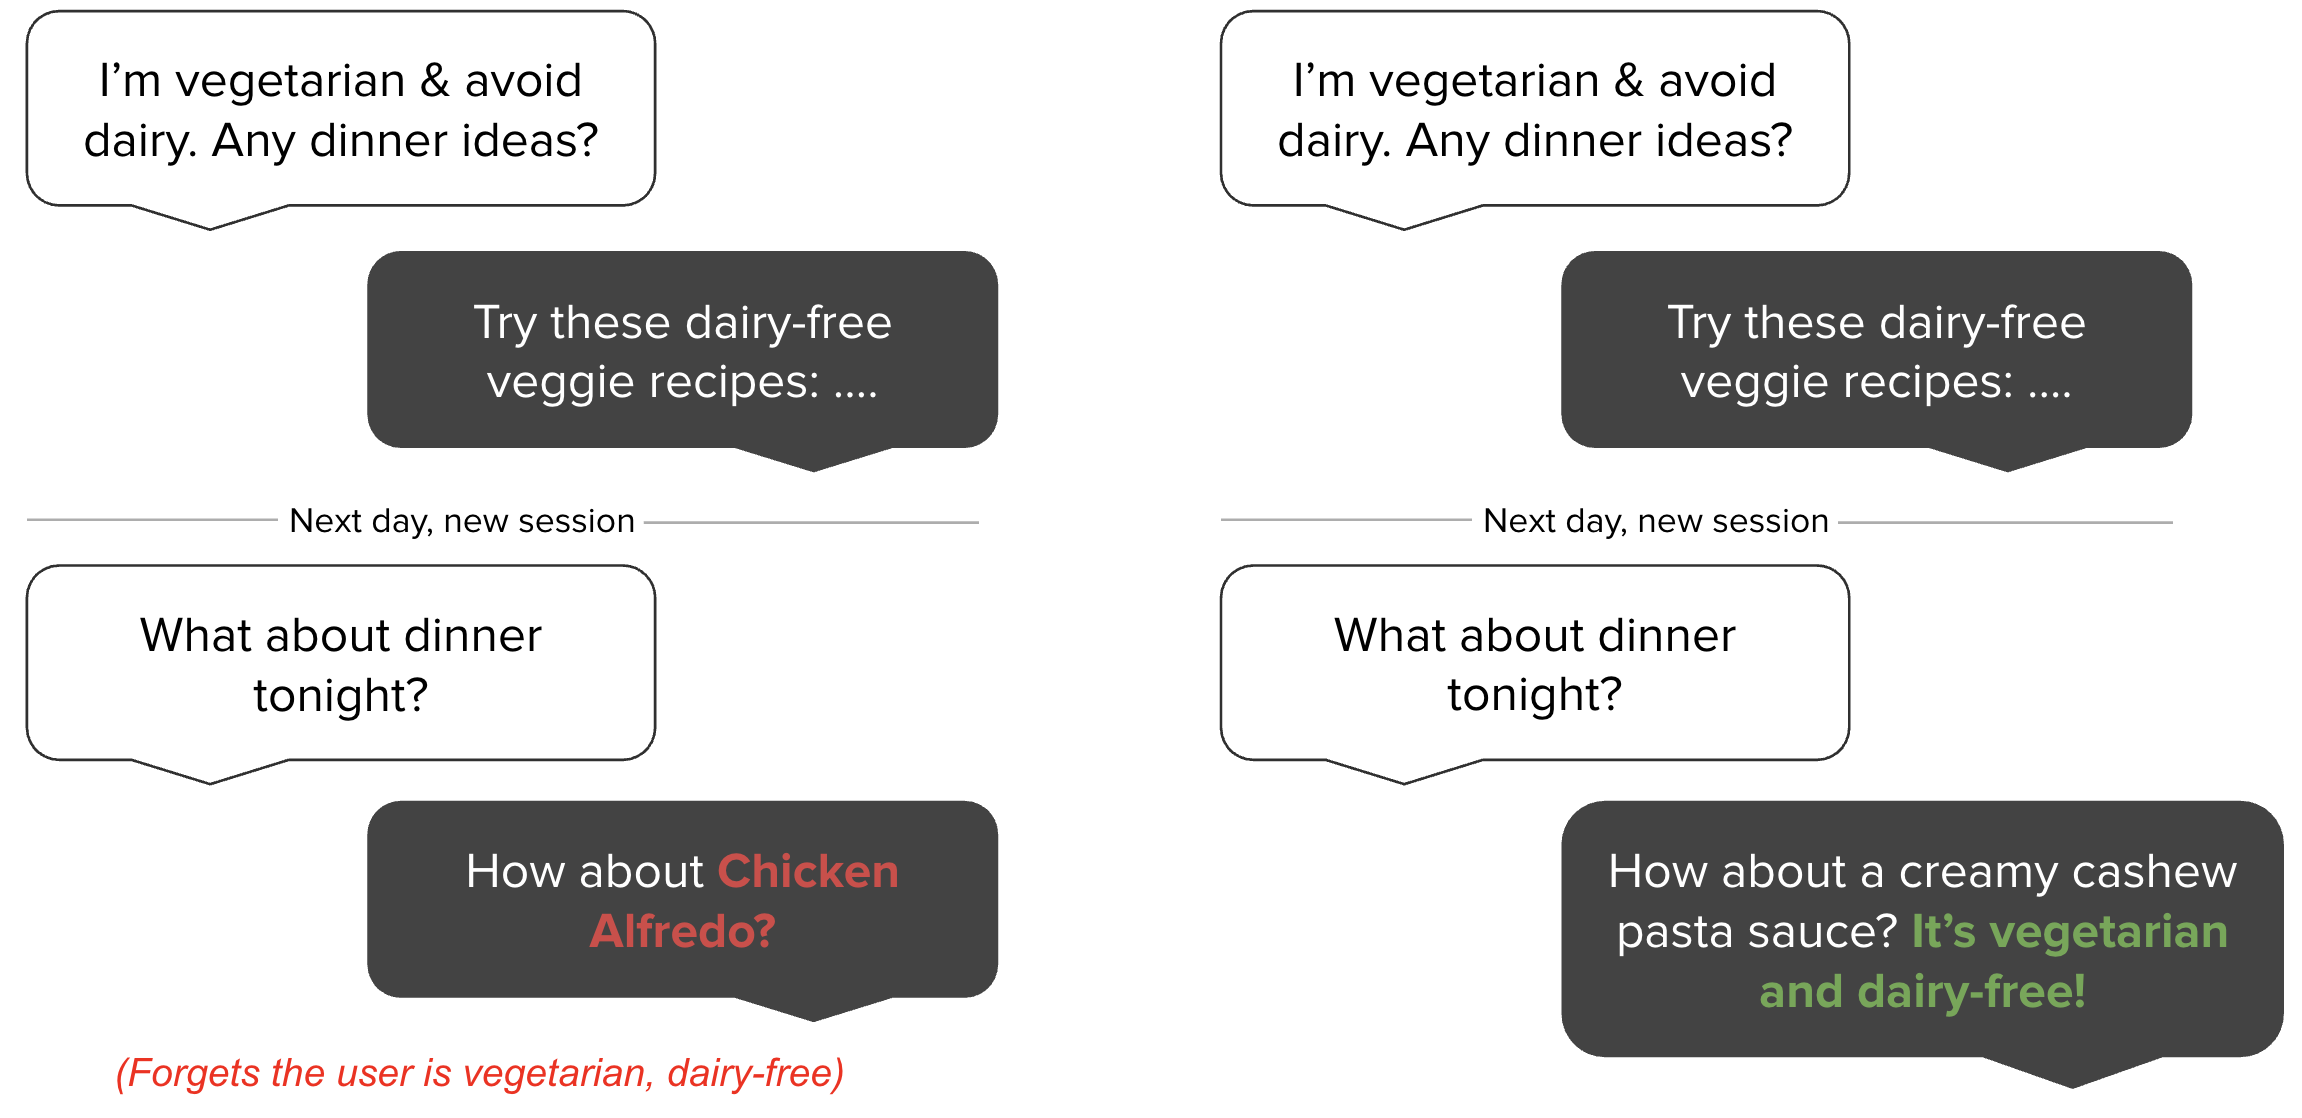
\includegraphics[width=\textwidth]{figures/main_figure.png}
    \end{minipage}%
    \hfill
    \begin{minipage}[t]{0.32\textwidth}
        \vspace{-5.3cm}
        \captionof{figure}{\textbf{Illustration of memory importance in AI agents.} 
        \textit{Left}: Without persistent memory, the system forgets critical user information (vegetarian, dairy-free preferences) between sessions, resulting in inappropriate recommendations. 
        \textit{Right}: With effective memory, the system maintains these dietary preferences across interactions, enabling contextually appropriate suggestions that align with previously established constraints.}
        \label{fig:main}
    \end{minipage}
\end{figure}


Unlike humans, who dynamically integrate new information and revise outdated beliefs, LLMs effectively ``\textit{reset}" once information falls outside their context window \citep{zhang2024guided, timoneda2025memory}. 
Even as models like OpenAI's GPT-4 (128K tokens) \citep{hurst2024gpt}, o1 (200K context) \citep{jaech2024openai}, Anthropic's Claude 3.7 Sonnet (200K tokens) \citep{anthropic2023modelcard}, and Google's Gemini (at least 10M tokens) \citep{team2024gemini} push the boundaries of context length, these improvements merely delay rather than solve the fundamental limitation.
 In practical applications, even these extended context windows prove insufficient for two critical reasons. First, as meaningful human-AI relationships develop over weeks or months, conversation history inevitably exceeds even the most generous context limits. Second, and perhaps more importantly, real-world conversations rarely maintain thematic continuity. A user might mention dietary preferences (being vegetarian), then engage in hours of unrelated discussion about programming tasks, before returning to food-related queries about dinner options. In such scenarios, a full-context approach would need to reason through mountains of irrelevant information, with the critical dietary preferences potentially buried among thousands of tokens of coding discussions. Moreover, simply presenting longer contexts does not ensure effective retrieval or utilization of past information, as attention mechanisms degrade over distant tokens \citep{guo2024active, nelson2024needle}.
 This limitation is particularly problematic in high-stakes domains such as healthcare, education, and enterprise support, where maintaining continuity and trust is crucial \citep{hatalis2023memory}. To address these challenges, AI agents must adopt memory systems that go beyond static context extension. A robust AI memory should selectively store important information, consolidate related concepts, and retrieve relevant details when needed—\emph{mirroring human cognitive processes} \citep{he2024human}. By integrating such mechanisms, we can develop AI agents that maintain consistent personas, track evolving user preferences, and build upon prior exchanges. This shift will transform AI from transient, forgetful responders into reliable, long-term collaborators, fundamentally redefining the future of conversational intelligence.


In this paper, we address a fundamental limitation in AI systems: their inability to maintain coherent reasoning across extended conversations across different sessions, which severely restricts meaningful long-term interactions with users. We introduce \mem~(pronounced as \emph{mem-zero}), a novel memory architecture that dynamically captures, organizes, and retrieves salient information from ongoing conversations. Building on this foundation, we develop \memp, which enhances the base architecture with graph-based memory representations to better model complex relationships between conversational elements. 
Our experimental results on the \texttt{LOCOMO} benchmark demonstrate that our approaches consistently outperform existing memory systems—including memory-augmented architectures, retrieval-augmented generation (RAG) methods, and both open-source and proprietary solutions—across diverse question types, while simultaneously requiring significantly lower computational resources.
Latency measurements further reveal that \mem~operates with 91\% lower response times than full-context approaches, striking an optimal balance between sophisticated reasoning capabilities and practical deployment constraints. These contributions represent a meaningful step toward AI systems that can maintain coherent, context-aware conversations over extended durations—mirroring human communication patterns and opening new possibilities for applications in personal tutoring, healthcare, and personalized assistance.